%======================================================================
% CAPITULO 7: CONFIGURACION AVANZADA
%======================================================================

\chapter{Configuracion Avanzada}
\label{ch:configuracion}

Este capitulo describe las opciones de configuracion avanzada de \sdc{}, incluyendo personalizacion visual, ajustes de red, control de acceso y gestion de actualizaciones.

\section{Temas Visuales}
\label{sec:temas}

SDC ofrece multiples temas visuales para adaptarse a las preferencias del usuario y condiciones de uso.

\begin{figure}[H]
\centering
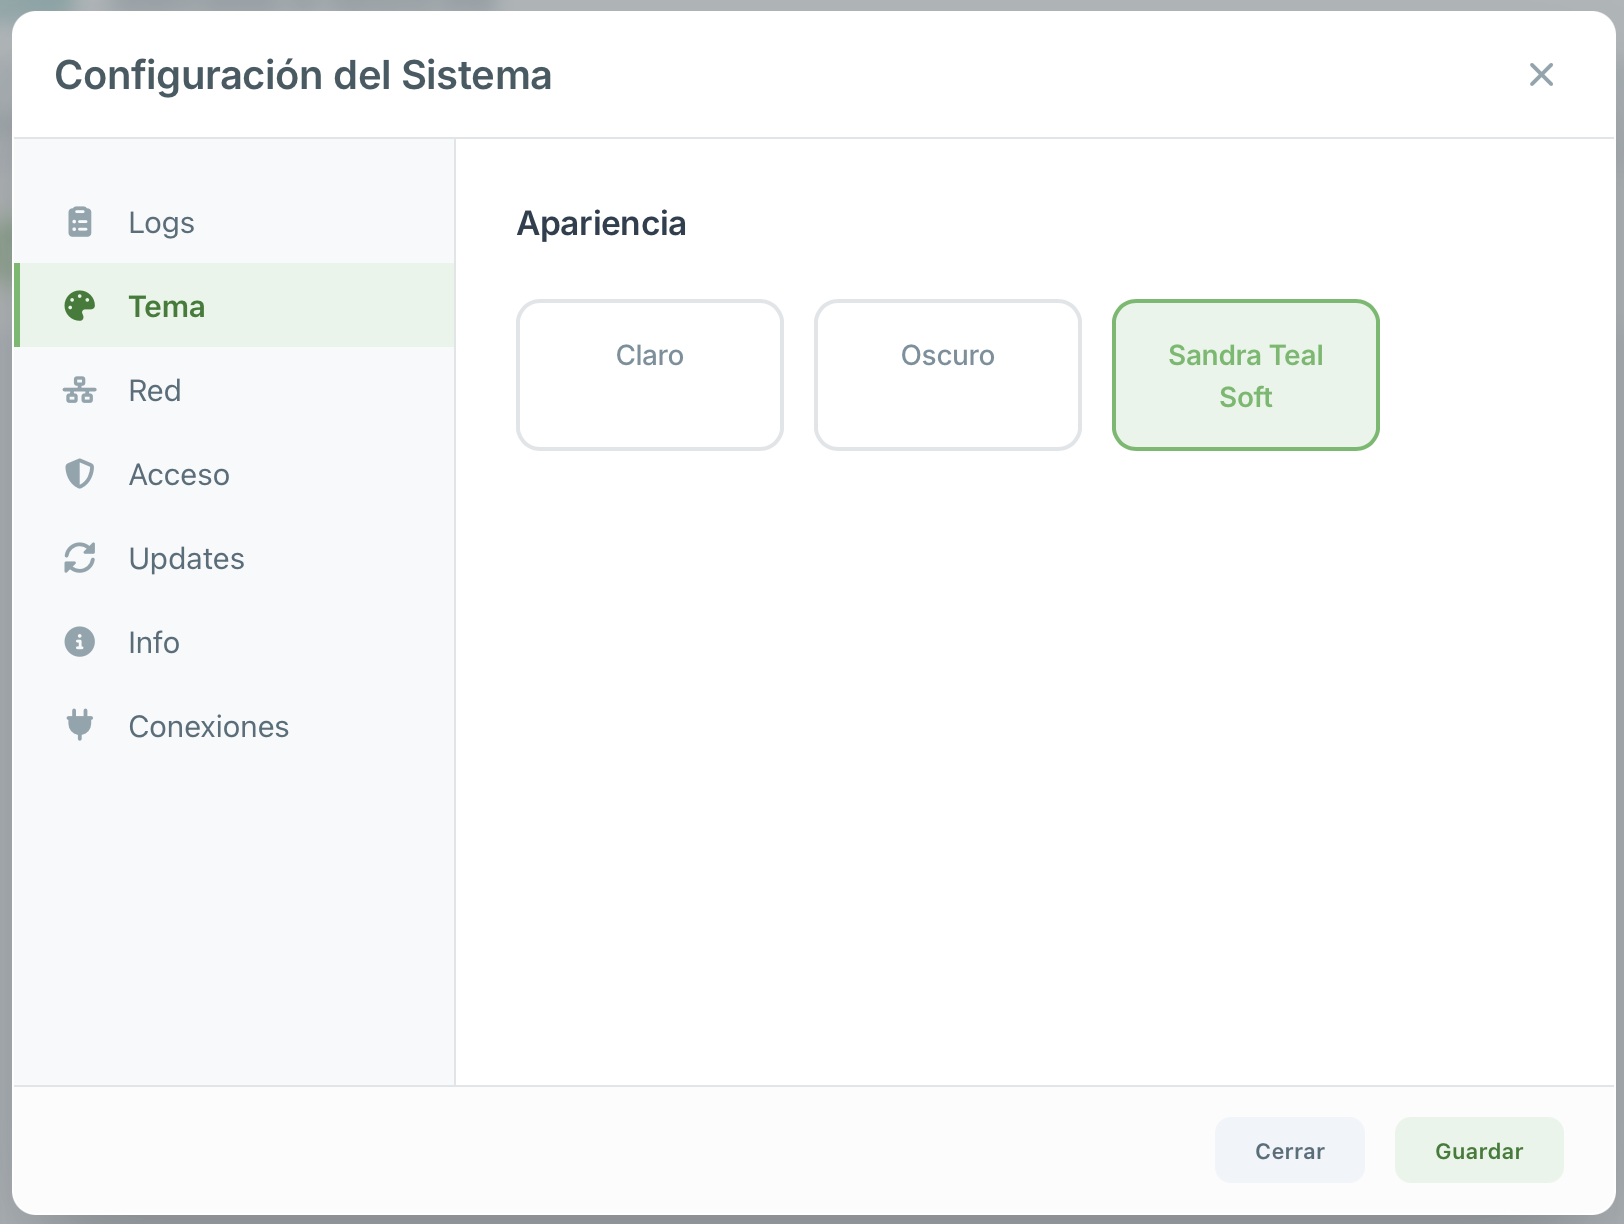
\includegraphics[width=0.95\textwidth]{anexos/17 temas.png}
\caption{Selector de temas visuales}
\label{fig:temas}
\end{figure}

\subsection{Temas Disponibles}

\begin{table}[H]
\centering
\begin{tabular}{p{3.5cm}p{4cm}p{5.5cm}}
\toprule
\textbf{Tema} & \textbf{Caracteristicas} & \textbf{Mejor Para} \\
\midrule
\textbf{Sandra Teal Soft} & Paleta verde agua suave, contraste moderado & Uso diurno, oficinas \\
\midrule
\textbf{Tema Oscuro} & Fondo oscuro, texto claro, menos fatiga visual & Uso nocturno, habitaciones oscuras \\
\midrule
\textbf{Alto Contraste} & Colores saturados, bordes definidos & Accesibilidad, proyecciones \\
\midrule
\textbf{Minimalista} & Elementos reducidos, mas espacio libre & Pantallas pequenas, foco en contenido \\
\bottomrule
\end{tabular}
\caption{Temas visuales disponibles en SDC}
\label{tab:temas}
\end{table}

\subsection{Ajustes de Personalizacion}

Ademas del tema base, se pueden personalizar:

\begin{itemize}[leftmargin=*]
    \item \textbf{Tamano de Fuente}: Pequeno, Normal, Grande, Extra Grande
    \item \textbf{Espaciado}: Compacto, Normal, Espaciado
    \item \textbf{Animaciones}: Activadas, Reducidas, Desactivadas
    \item \textbf{Efectos de Transparencia}: Nivel de opacidad de paneles flotantes
    \item \textbf{Color de Acento}: Personalizar el color principal de la interfaz
\end{itemize}

\begin{quote}
\textbf{Sincronizacion de Preferencias}\\
Las preferencias visuales se sincronizan automaticamente entre sesiones mediante el Client ID, garantizando una experiencia consistente en multiples dispositivos.
\end{quote}

\section{Configuracion de Red}
\label{sec:red}

El panel de configuracion de red permite ajustar parametros avanzados de conectividad.

\begin{figure}[H]
\centering
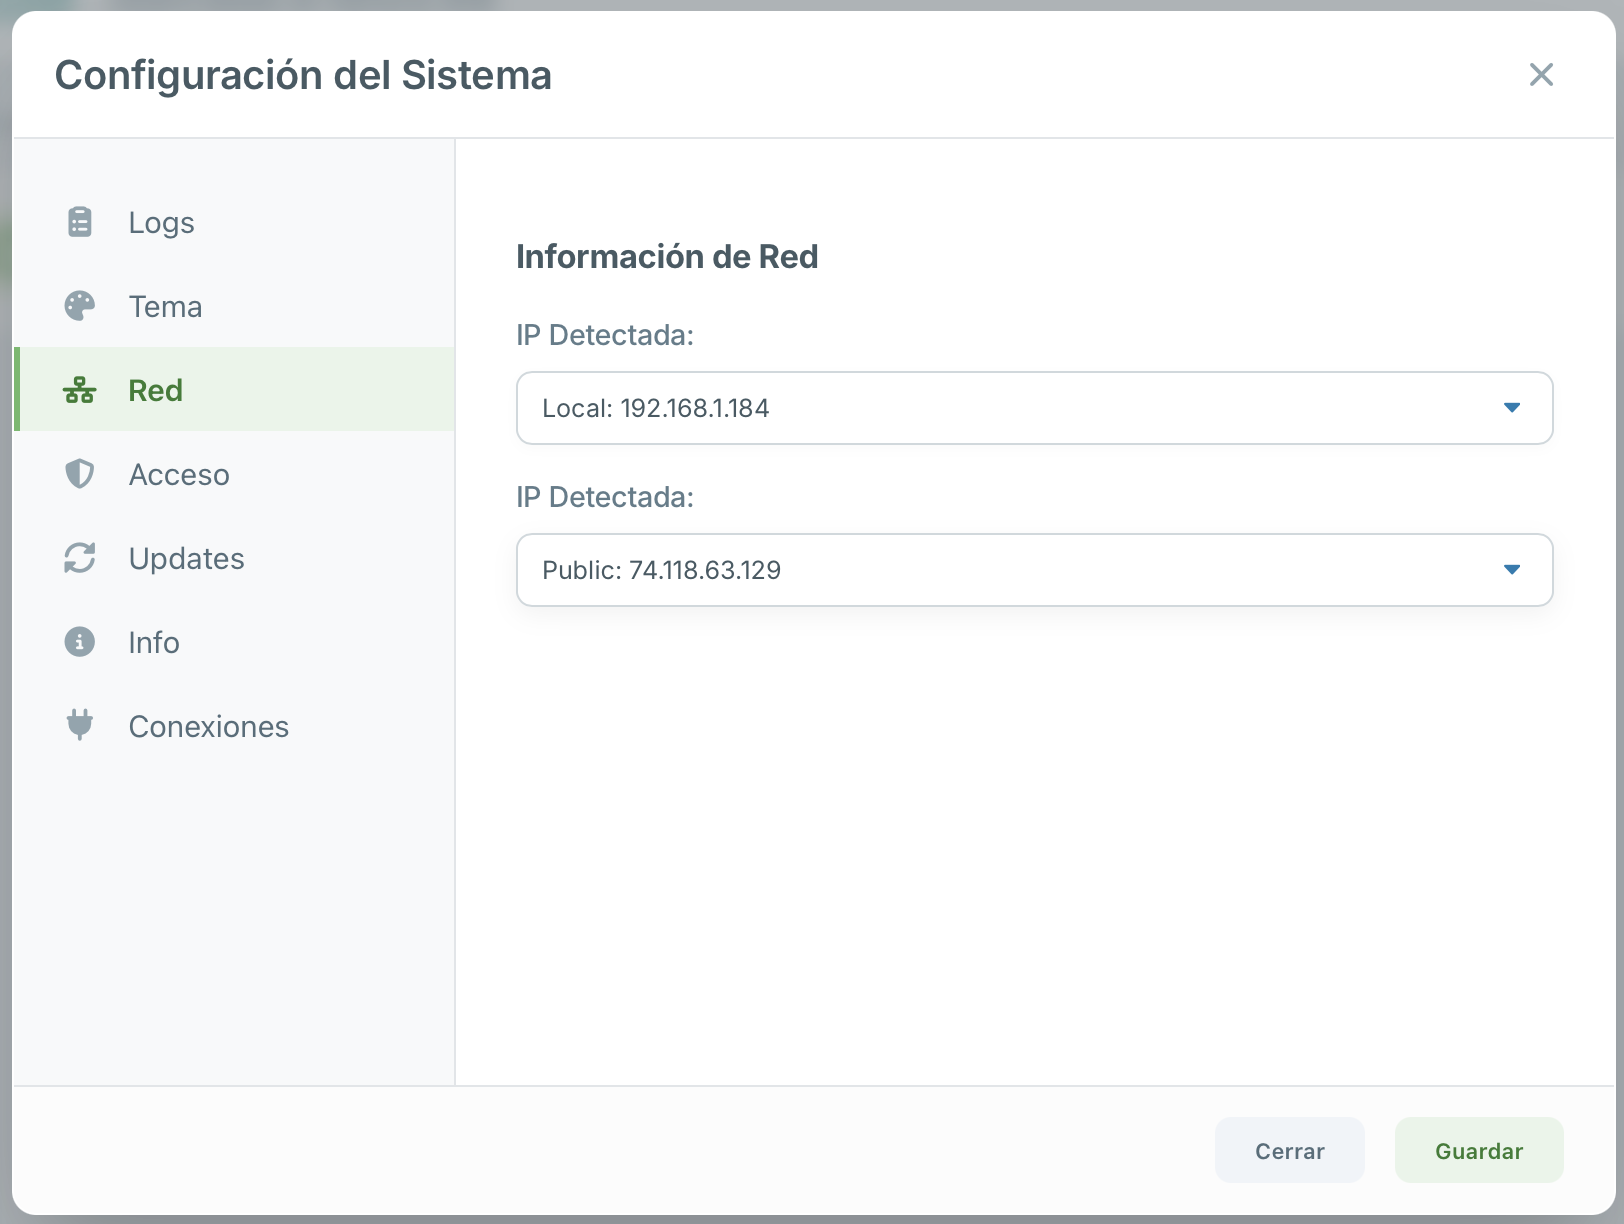
\includegraphics[width=0.95\textwidth]{anexos/18 red.png}
\caption{Configuracion avanzada de red}
\label{fig:red}
\end{figure}

\subsection{Parametros de Conexion}

\begin{table}[H]
\centering
\begin{tabular}{p{4.5cm}p{3cm}p{5.5cm}}
\toprule
\textbf{Parametro} & \textbf{Valor Default} & \textbf{Descripcion} \\
\midrule
Timeout de Conexion & 30 segundos & Tiempo maximo para establecer conexion \\
\midrule
Reintentos Automaticos & 3 intentos & Numero de reintentos ante fallo \\
\midrule
Intervalo de Keep-Alive & 60 segundos & Frecuencia de pings de mantenimiento \\
\midrule
Compresion de Datos & Activada & Reduce uso de ancho de banda \\
\midrule
Buffer de Red & 64 KB & Tamano del buffer de transmision \\
\bottomrule
\end{tabular}
\caption{Parametros configurables de red}
\label{tab:config-red}
\end{table}

\subsection{Configuracion de Proxy}

SDC soporta multiples configuraciones de proxy:

\begin{itemize}[leftmargin=*]
    \item \textbf{Proxy HTTP/HTTPS}: Configuracion estandar para trafico web
    \item \textbf{Proxy SOCKS5}: Para aplicaciones que requieren capa de transporte
    \item \textbf{Proxy Automatico (PAC)}: Deteccion automatica mediante script
    \item \textbf{Proxy por Aplicacion}: Cada app puede tener su propia configuracion
\end{itemize}

\subsection{Politicas de DNS}

\begin{quote}
\textbf{Resolucion DNS Segura}\\
SDC implementa DNS sobre HTTPS (DoH) y DNS sobre TLS (DoT) para prevenir ataques de envenenamiento de cache DNS y garantizar la privacidad de las consultas.
\end{quote}

\section{Control de Acceso}
\label{sec:acceso}

El sistema de control de acceso permite definir quien puede hacer que dentro de SDC.

\begin{figure}[H]
\centering
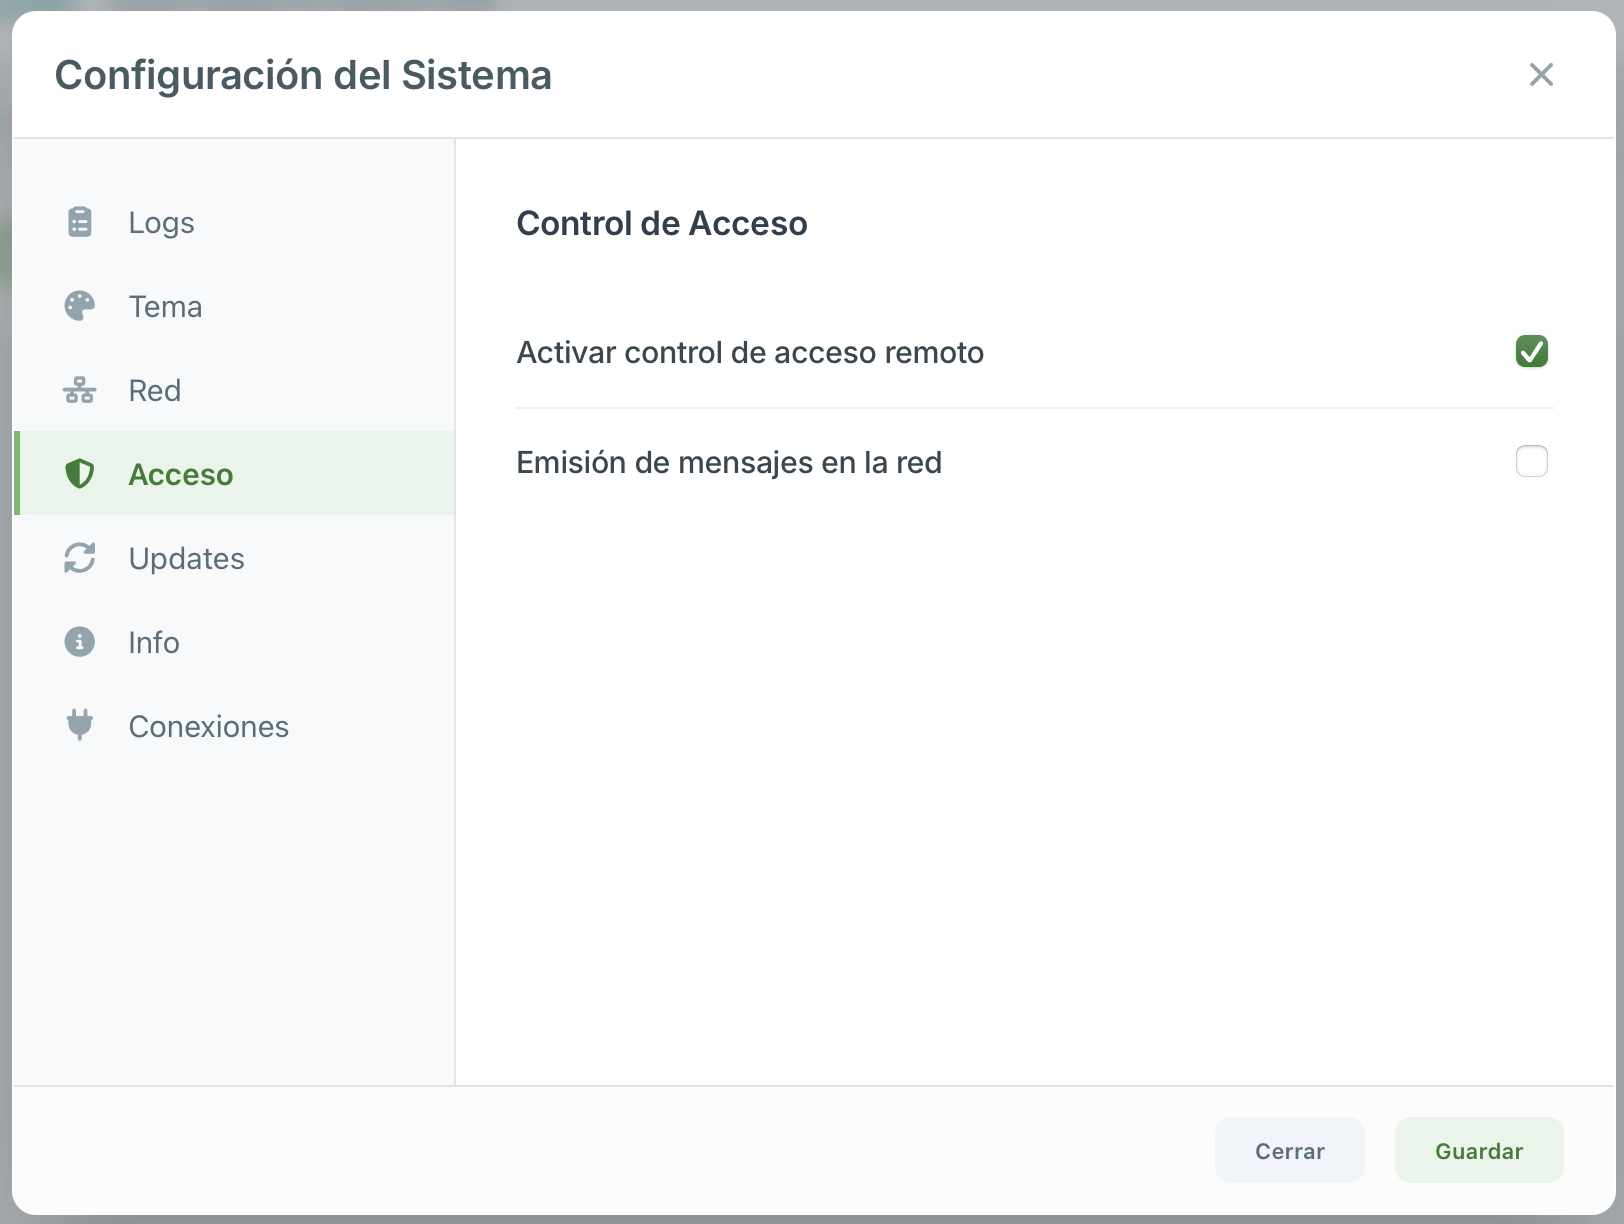
\includegraphics[width=0.95\textwidth]{anexos/19 acceso.png}
\caption{Panel de control de acceso}
\label{fig:acceso}
\end{figure}

\subsection{Niveles de Permisos}

\begin{table}[H]
\centering
\begin{tabular}{p{3cm}p{9.5cm}}
\toprule
\textbf{Nivel} & \textbf{Permisos} \\
\midrule
\textbf{Administrador} & Acceso total: configuracion del sistema, gestion de usuarios, auditoria completa, modificacion de politicas de seguridad \\
\midrule
\textbf{Operador} & Gestion de aplicaciones y conexiones, visualizacion de logs propios, uso de todas las herramientas excepto configuracion avanzada \\
\midrule
\textbf{Usuario} & Uso de aplicaciones asignadas, visualizacion de documentos autorizados, acceso limitado a metricas del sistema \\
\midrule
\textbf{Invitado} & Acceso temporal a aplicaciones publicas, sin capacidad de instalar o configurar \\
\bottomrule
\end{tabular}
\caption{Niveles de permisos de acceso}
\label{tab:niveles-acceso}
\end{table}

\subsection{Autenticacion Multifactor}

SDC soporta autenticacion adicional mediante:

\begin{itemize}[leftmargin=*]
    \item \textbf{Codigos TOTP}: Aplicaciones como Google Authenticator o Authy
    \item \textbf{Claves FIDO2/U2F}: Dispositivos fisicos como YubiKey
    \item \textbf{Biometria}: Huella dactilar o reconocimiento facial (segun hardware)
    \item \textbf{Tokens de Hardware}: Tarjetas inteligentes, certificados en USB
\end{itemize}

\section{Sistema de Actualizaciones}
\label{sec:updates}

El gestor de actualizaciones mantiene SDC al dia con las ultimas mejoras y parches de seguridad.

\begin{figure}[H]
\centering
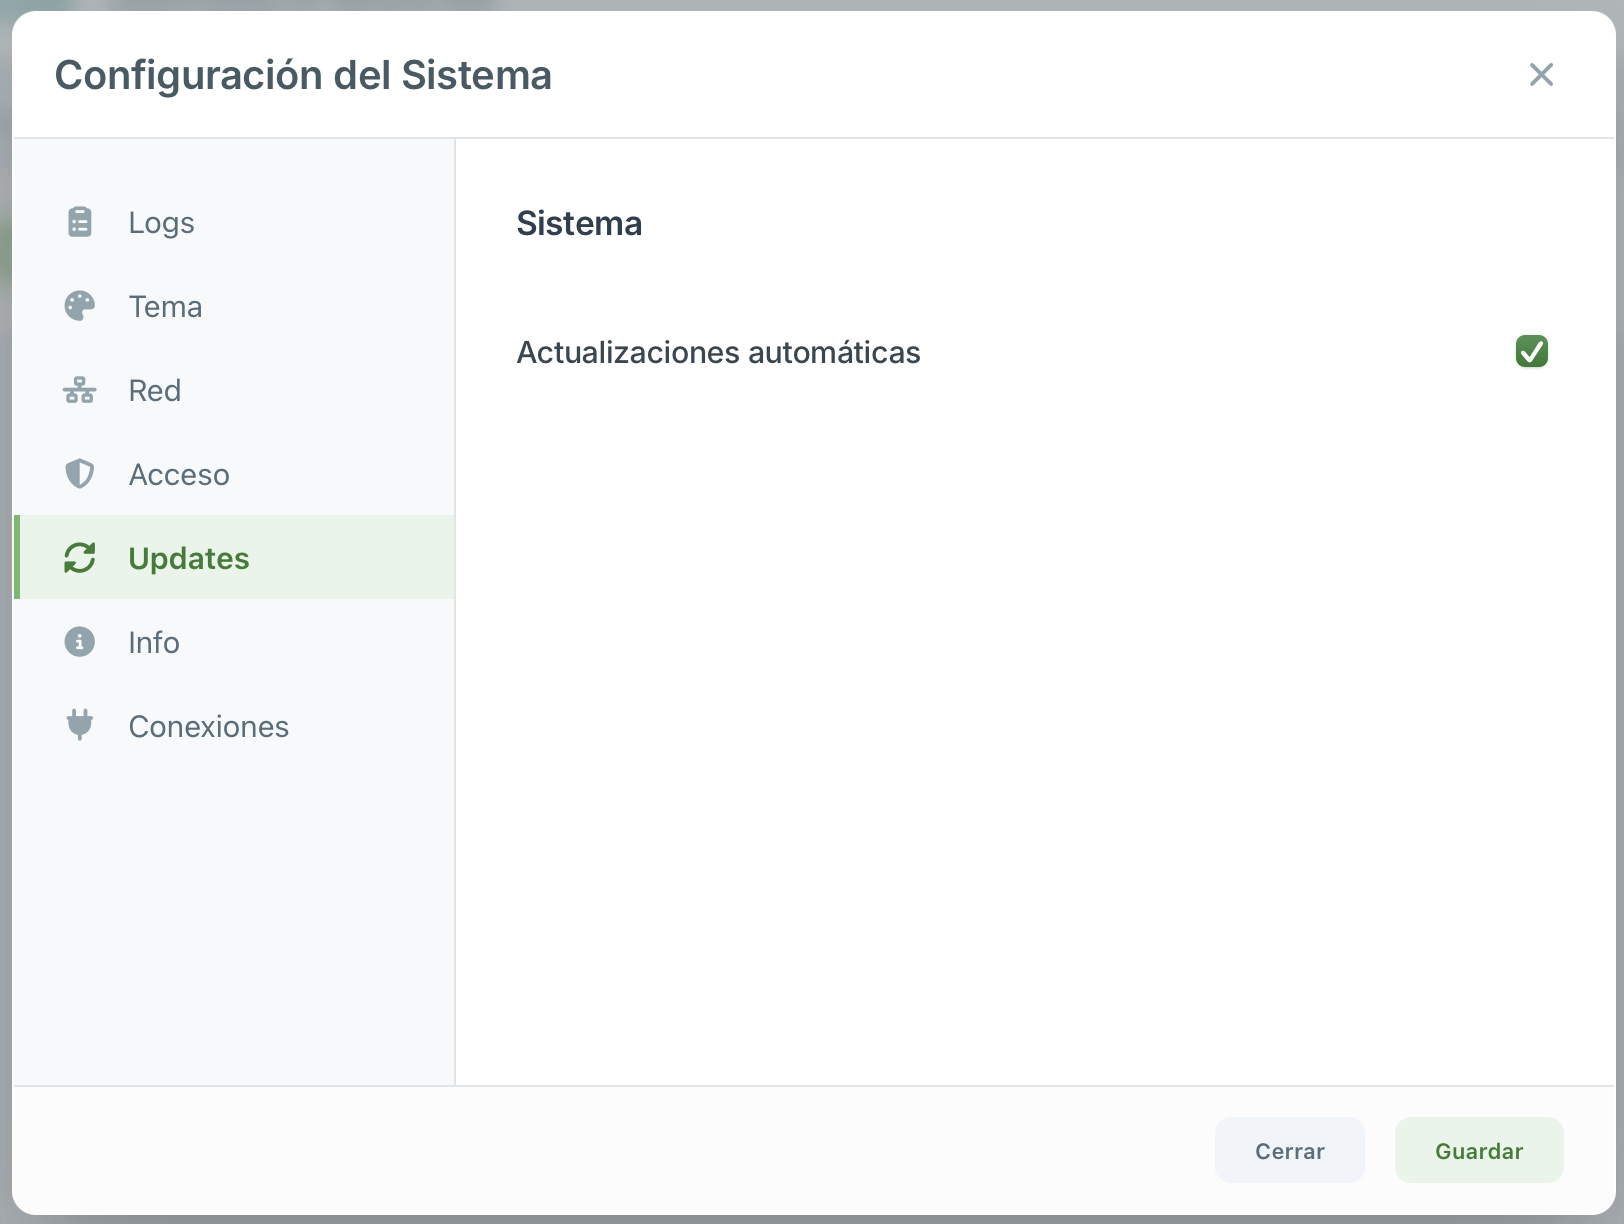
\includegraphics[width=0.95\textwidth]{anexos/20 updates.png}
\caption{Gestor de actualizaciones}
\label{fig:updates}
\end{figure}

\subsection{Canales de Actualizacion}

\begin{table}[H]
\centering
\begin{tabular}{p{3cm}p{4cm}p{5.5cm}}
\toprule
\textbf{Canal} & \textbf{Estabilidad} & \textbf{Recomendado Para} \\
\midrule
Stable & Alta & Entornos de produccion \\
\midrule
Beta & Media & Testing y desarrollo \\
\midrule
Nightly & Baja & Usuarios avanzados, QA \\
\midrule
LTS & Muy Alta & Sistemas criticos, compliance \\
\bottomrule
\end{tabular}
\caption{Canales de actualizacion disponibles}
\label{tab:canales-updates}
\end{table}

\subsection{Tipos de Actualizacion}

\begin{itemize}[leftmargin=*]
    \item \textbf{Actualizaciones de Seguridad}: Parches criticos (instalacion automatica recomendada)
    \item \textbf{Actualizaciones de Funciones}: Nuevas capacidades (instalacion manual)
    \item \textbf{Actualizaciones de Aplicaciones}: Nueva version de apps desplegadas
    \item \textbf{Definiciones de Seguridad}: Firmas antivirus, listas de bloqueo (automatico)
\end{itemize}

\begin{quote}
\textbf{Rollback de Actualizaciones}\\
Si una actualizacion causa problemas, SDC permite revertir a la version anterior automaticamente mediante el sistema de instantaneas (snapshots). El proceso toma menos de 2 minutos.
\end{quote}

\section{Informacion del Sistema}
\label{sec:info}

El panel de informacion del sistema proporciona datos tecnicos detallados sobre la instalacion actual.

\begin{figure}[H]
\centering
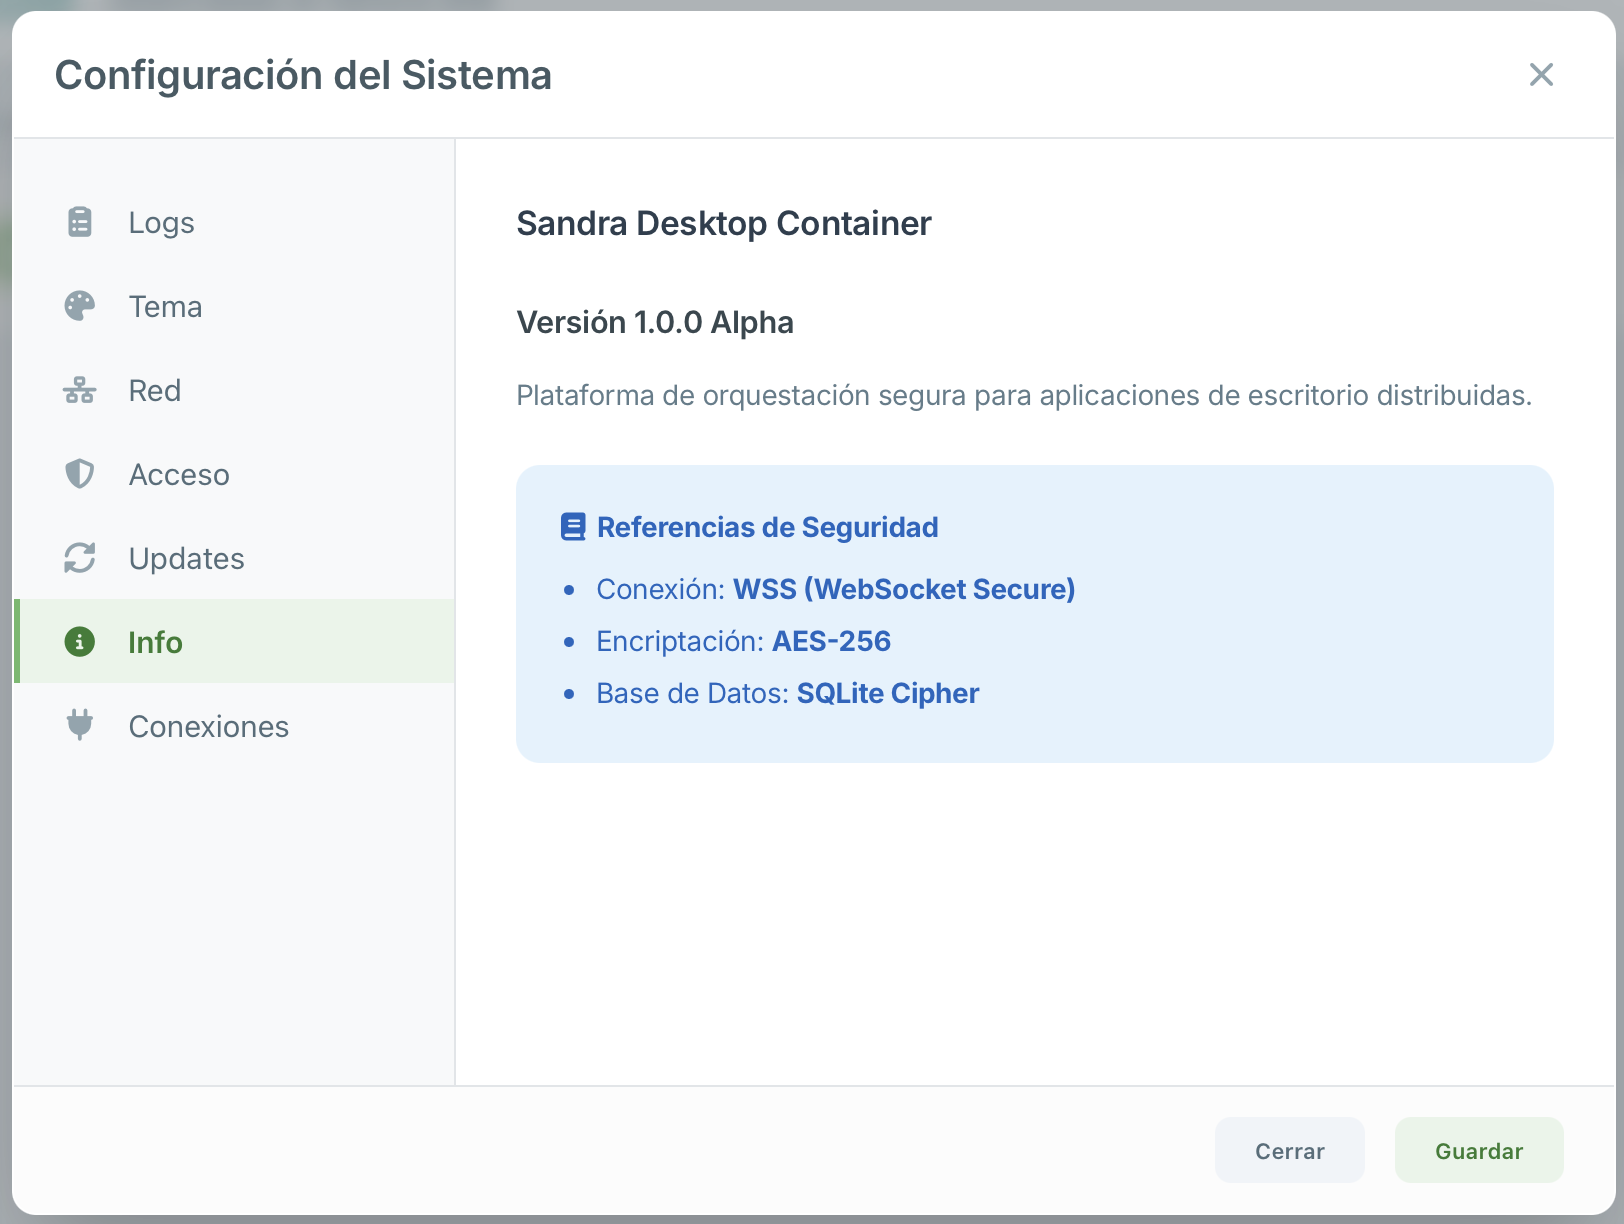
\includegraphics[width=0.95\textwidth]{anexos/21 info.png}
\caption{Informacion detallada del sistema}
\label{fig:info}
\end{figure}

\subsection{Datos Tecnicos Mostrados}

\begin{table}[H]
\centering
\begin{tabular}{p{4cm}p{9cm}}
\toprule
\textbf{Categoria} & \textbf{Informacion} \\
\midrule
\textbf{Version} & Numero de version de SDC, build date, commit hash \\
\midrule
\textbf{Runtime} & Version de Rust, Angular, Tauri, SQLite \\
\midrule
\textbf{Hardware} & CPU, RAM, almacenamiento, interfaces de red \\
\midrule
\textbf{Licencia} & Tipo de licencia, fecha de expiracion, caracteristicas habilitadas \\
\midrule
\textbf{Registro} & Client ID, fecha de instalacion, ultimo acceso \\
\bottomrule
\end{tabular}
\caption{Datos tecnicos del sistema}
\label{tab:datos-sistema}
\end{table}

\subsection{Exportacion de Diagnostico}

Para soporte tecnico, SDC puede generar un paquete de diagnostico que incluye:

\begin{itemize}[leftmargin=*]
    \item Logs del sistema (sin datos sensibles)
    \item Configuracion actual (anonimizada)
    \item Estado de componentes
    \item Historial de errores recientes
    \item Metricas de rendimiento
\end{itemize}

\begin{quote}
\textbf{Privacidad del Diagnostico}\\
Antes de generar el paquete de diagnostico, SDC permite revisar y excluir informacion que pueda considerarse sensible. Nunca se incluyen contrasenas, claves privadas o contenido de documentos.
\end{quote}

\section{Cierre del Sistema}
\label{sec:cierre}

El cierre seguro de SDC garantiza que todos los datos sensibles se protejan adecuadamente.

\begin{figure}[H]
\centering
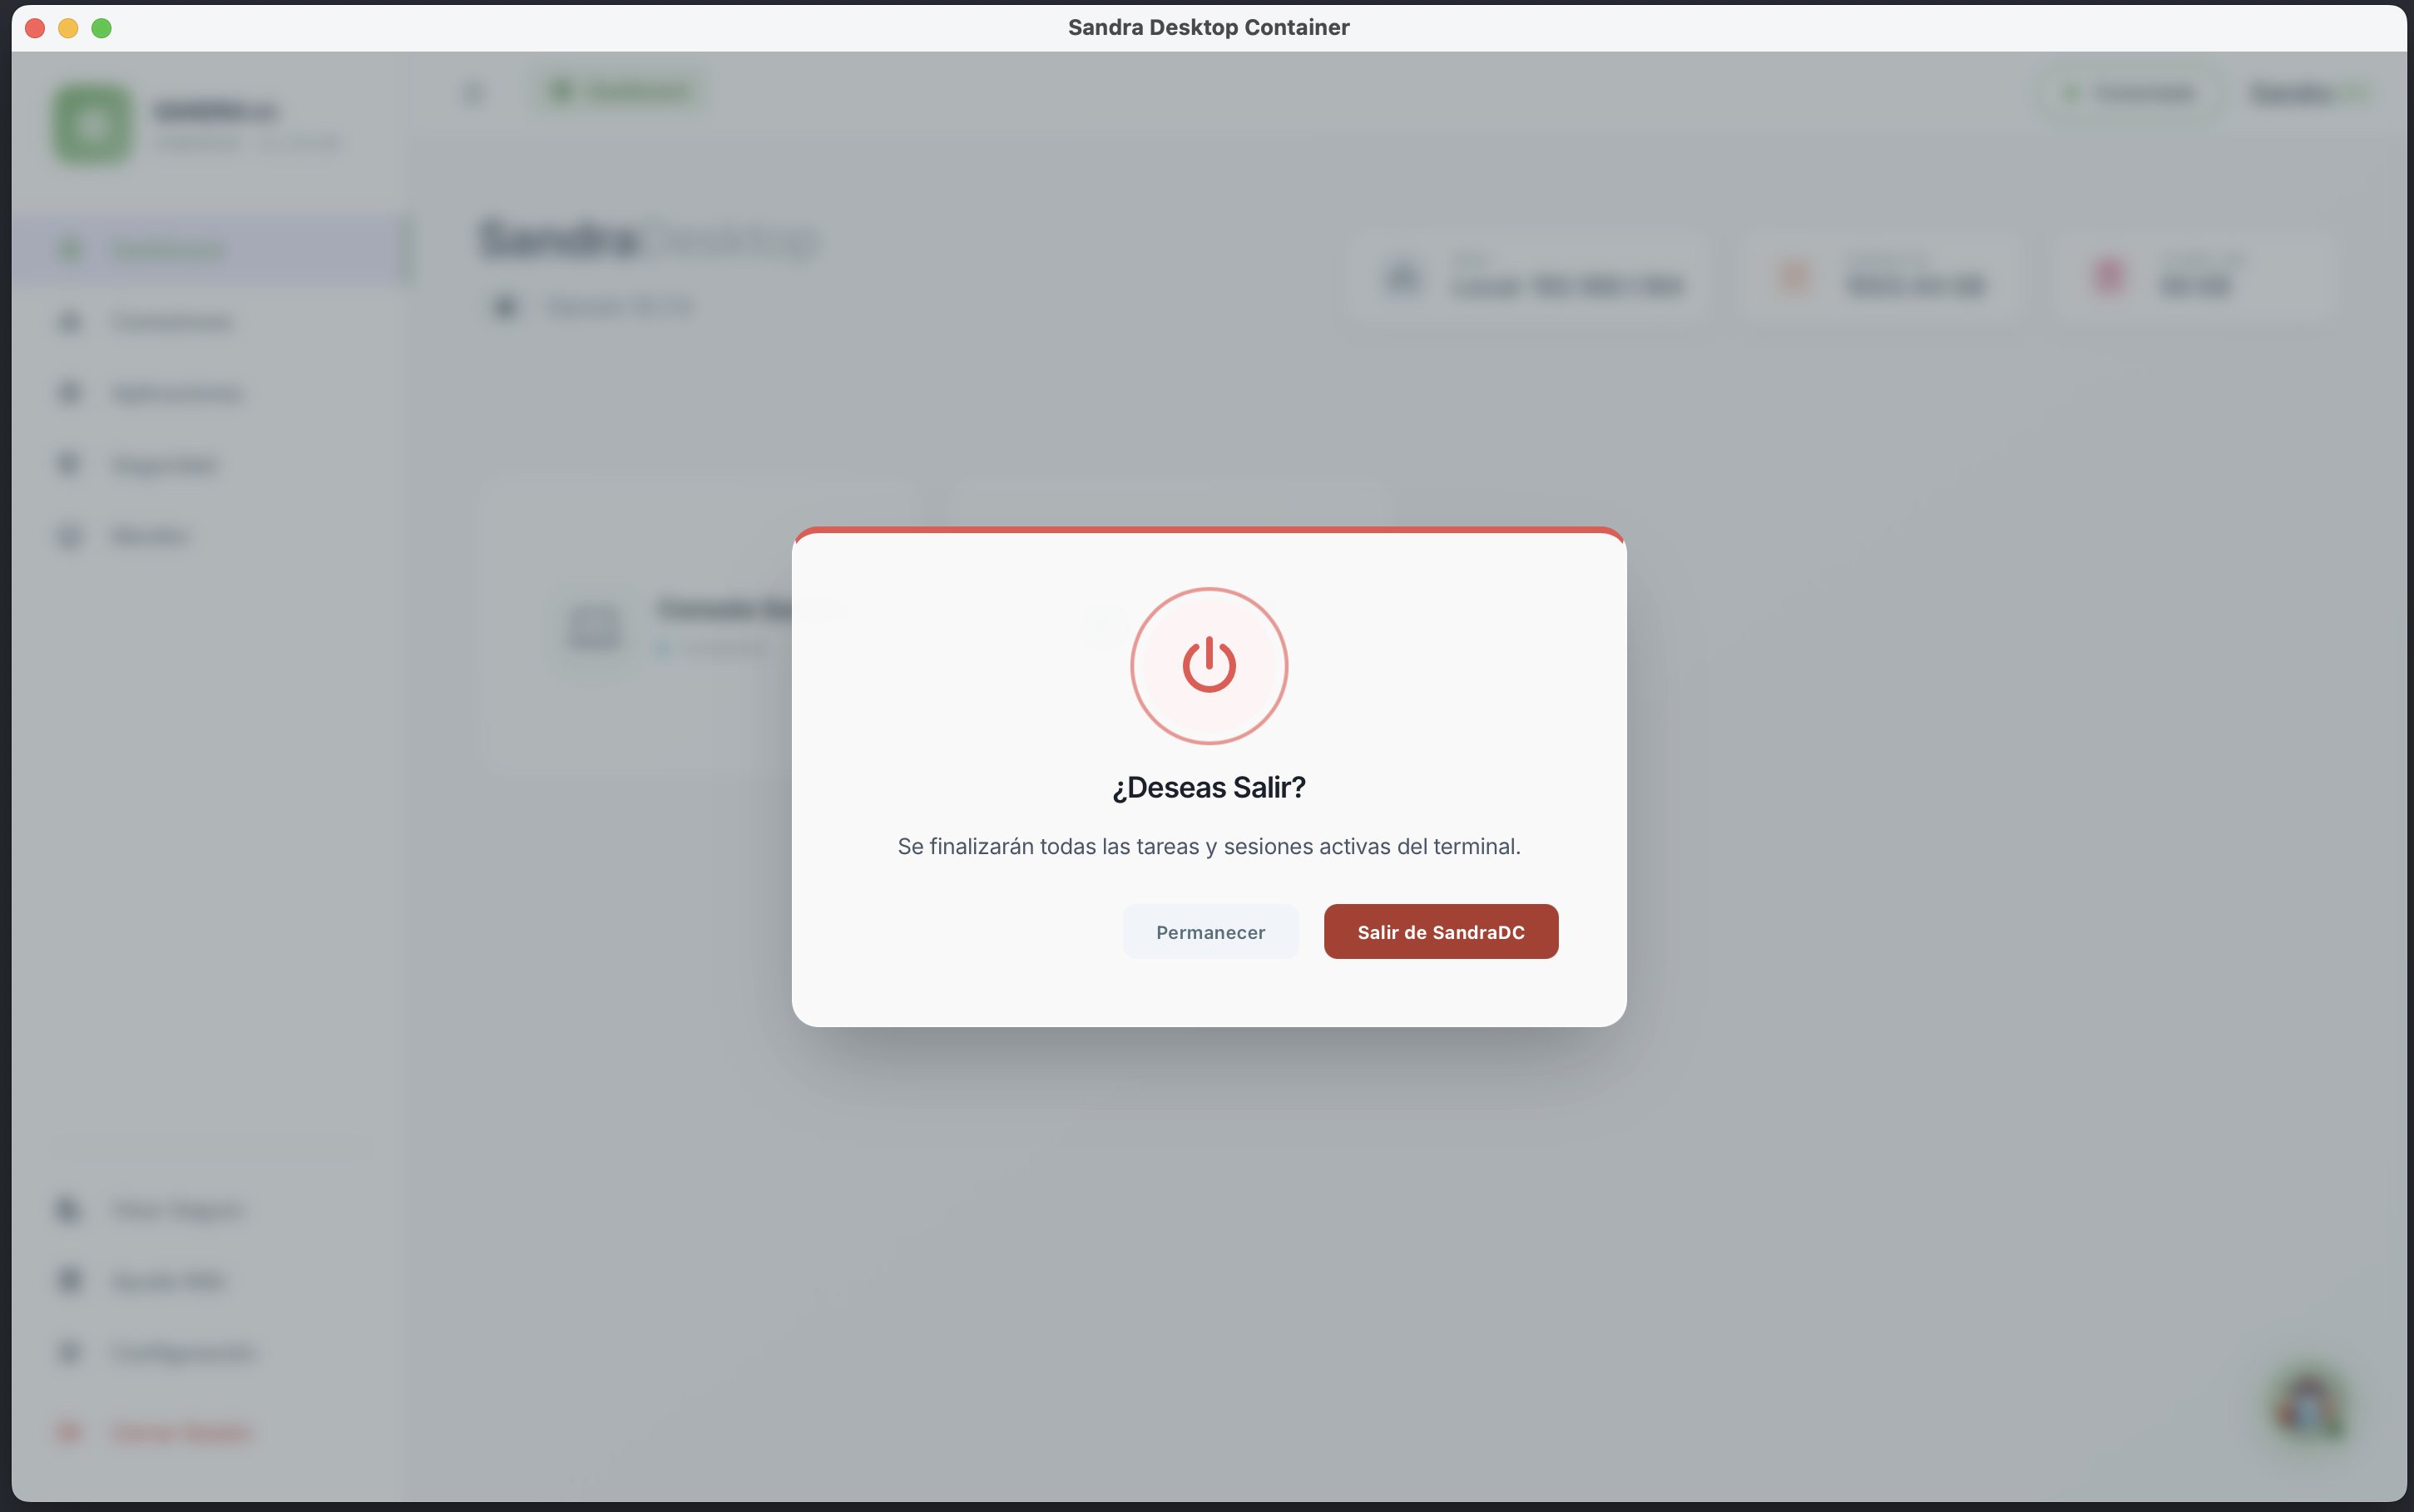
\includegraphics[width=0.95\textwidth]{anexos/fin sistema.png}
\caption{Pantalla de cierre del sistema}
\label{fig:cierre}
\end{figure}

\subsection{Procedimiento de Cierre}

Al cerrar SDC, el sistema realiza automaticamente:

\begin{enumerate}[leftmargin=*]
    \item \textbf{Limpieza de Memoria}: Todos los buffers de documentos abiertos se sobreescriben con ceros
    \item \textbf{Cierre de Conexiones}: Las conexiones activas se cierran ordenadamente
    \item \textbf{Persistencia de Estado}: La configuracion y preferencias se guardan en la base de datos
    \item \textbf{Bloqueo de Sesion}: El Client ID se marca como inactivo hasta el proximo inicio
    \item \textbf{Registro de Auditoria}: Se registra el evento de cierre con timestamp y duracion de la sesion
\end{enumerate}

\subsection{Opciones de Cierre}

\begin{table}[H]
\centering
\begin{tabular}{p{4cm}p{8.5cm}}
\toprule
\textbf{Opcion} & \textbf{Descripcion} \\
\midrule
Cierre Normal & Cierra aplicaciones de forma ordenada, guarda todo \\
\midrule
Cierre Rapido & Fuerza cierre inmediato, riesgo minimo de perdida de datos \\
\midrule
Cierre y Bloqueo & Cierra SDC y bloquea la pantalla del sistema \\
\midrule
Cierre y Suspender & Cierra SDC y suspende el dispositivo \\
\bottomrule
\end{tabular}
\caption{Opciones de cierre disponibles}
\label{tab:opciones-cierre}
\end{table}

\begin{quote}
\textbf{Advertencia Importante}\\
Evita cerrar SDC forzosamente (matar el proceso) mientras tengas documentos sensibles abiertos en el visor. Esto podria comprometer la garantia de zero-fill de la memoria. Siempre usa el cierre ordenado mediante el menu o el boton de cierre seguro.
\end{quote}

\section{Mejores Practicas de Configuracion}

\begin{enumerate}[leftmargin=*]
    \item \textbf{Realiza Backups}: Exporta tu configuracion periodicamente antes de cambios mayores
    \item \textbf{Documenta Cambios}: Manten un registro de modificaciones para auditoria
    \item \textbf{Prueba en Desarrollo}: Valida configuraciones nuevas en entorno de pruebas primero
    \item \textbf{Revisa Actualizaciones}: Lee las notas de release antes de actualizar
    \item \textbf{Configura Alertas}: Activa notificaciones para eventos criticos del sistema
\end{enumerate}
